\subsection{Work Package 1: Formalized model-driven requirements engineering}

\subsubsection{Expected Result}

Techniques surrounding \ctextbf{Domain Specific Modeling Language (DSML)}:
\vspace{-.5cm}
\begin{itemize}
  \item AI-based error detection;
  \item formal verification;
  \item consistency and completeness analysis.
  \item model simulators: concerning the interactions with models' 
    surrounding environment;
  \item natural language processing: automated extraction procedure 
    of requirements written in natural languages.
\end{itemize}

\newcommand{\clanodetxt}[1]{\textbf{\footnotesize{#1}}}
\begin{figure}[H]
\centering  
\begin{tikzpicture}
  \tikzstyle{textnode}=[rectangle, draw = black]

  \node[textnode] (fpd) {\clanodetxt{Step 1: Syntax and Semantics of 
    Formalized Process Description}};

  \node[textnode] (pn) [below = of fpd] {\clanodetxt{Step 2.1: Description of 
    the model with Petri Net}}
    edge[<-] (fpd);
\end{tikzpicture}
\caption{Road map.}
\end{figure}

\subsubsection{Syntax and Semantics of Formalized Process Description}

\begin{itemize}
  \item process operators $O$,
  \item technical resources $T$,
  \item states $Z$ (product $P$ and energy $E$).
  \item relation 
\end{itemize}

\begin{align*}
  O &= \{O_1, O_2, \dots, O_n\} \\
  Z &= \{P_1, \dots, P_n, E_1, \dots, E_n\} \\
  T &= \{T_1, T_2, \dots, T_n\} \\
  F &\subseteq (O \times Z) \cup (Z \times O) \\
  U &\subseteq (O \times T) \\
\end{align*}

\subsubsection{Case study}

\begin{figure}
  \centering
  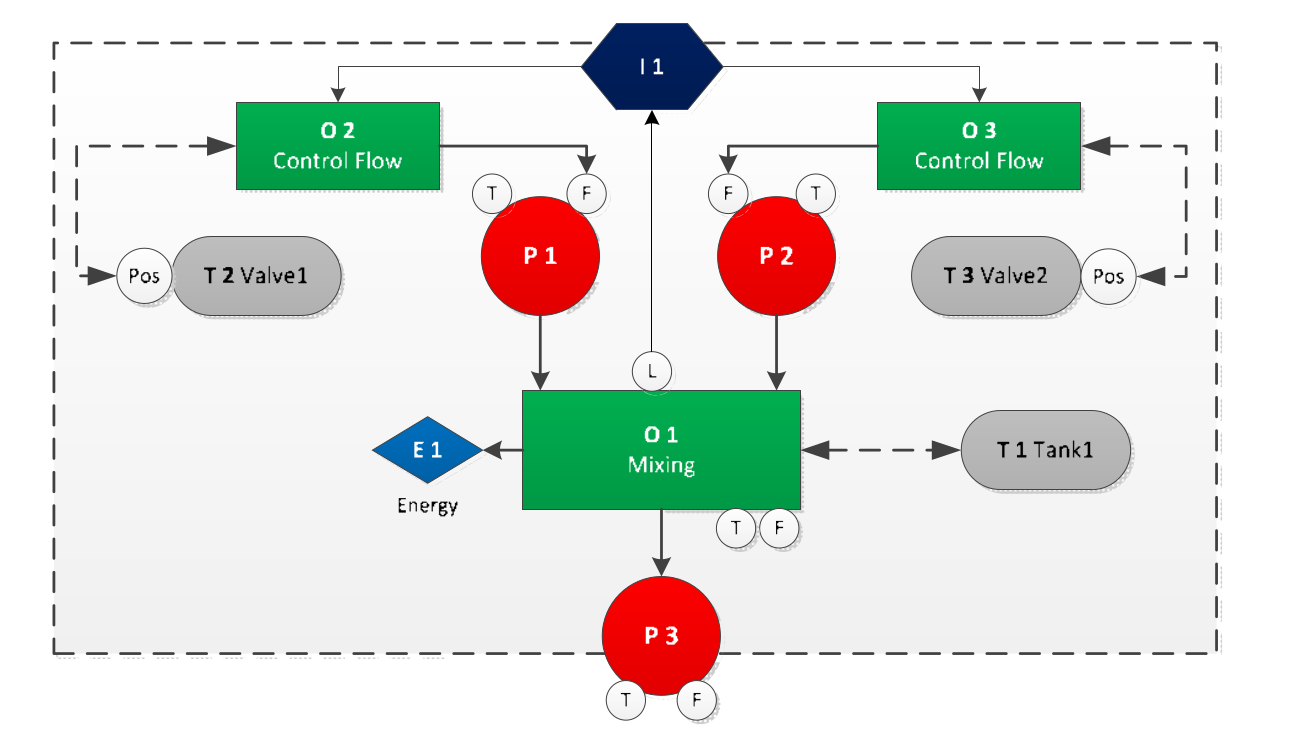
\includegraphics[width=.8\textwidth]{notes/project/AITOC-2020/img/FPB.png}
  \caption{A sample FPB}
\end{figure}

- Fig. 7 in paper {2011, Improved diagnosis by combining structural and process knowledge}
- use Cosmos ?
- logic ?

\textbf{Differential Logic description of FPB}

Cyber side, the operation blocks:

\begin{itemize}
  \item $I_i$: input
  \item $Eop$: operations
  \item $U_j$: update
\end{itemize}

\begin{align*}
  HP_{cyber} = \{?(I_0 \wedge I_1 \wedge \dots \wedge I_n);
    Eop; U_0; U_1; \dots; U_m\}  
\end{align*}

\begin{enumerate}
  \item Determine whether there exists a deadlock in the system 
    (consistency analysis).
  \item Correct behavior.
\end{enumerate}

